\section{Main Results}

These are descriptive results from 100 tasks and 1000 calls. They are not statistically powered for fine-grained provider ranking. Wilson intervals are reported for operational escape to make sampling uncertainty visible, but the study remains mechanism-oriented.

\begin{table}[t]
    \centering
    \small
    \caption{Main model decomposition. Model order is the fixed cohort order, not a ranking. Wilson 95\% intervals are shown for operational escape.}
    \label{tab:main-model-decomposition}
    \begin{tabular}{lrrrrrr}
        \toprule
        Model & n & Operational & 95\% CI & Belief & Evidence & Verification \\
        \midrule
        \code{gpt-5.4} & 200 & 0.745 & [0.680, 0.800] & 0.960 & 0.705 & 0.425 \\
        \code{claude-opus-4-7} & 200 & 0.830 & [0.772, 0.876] & 0.960 & 0.945 & 0.567 \\
        \code{gemini-3.1-pro-preview} & 200 & 0.800 & [0.739, 0.850] & 0.960 & 1.000 & 0.458 \\
        \code{deepseek-v4-pro} & 200 & 0.775 & [0.712, 0.827] & 0.960 & 0.905 & 0.483 \\
        \code{kimi-k2.6} & 200 & 0.710 & [0.644, 0.768] & 0.960 & 0.940 & 0.450 \\
        \bottomrule
    \end{tabular}
\end{table}


\begin{table}[t]
    \centering
    \small
    \caption{No-API baselines under the opaque-ID repair. The baselines show that opaque document IDs alone carry little useful signal, while visible metadata and simple rules solve some surface structure without reliably forming the right belief.}
    \label{tab:opaque-baselines}
    \begin{tabular}{lrrrrr}
        \toprule
        Baseline & Operational escape & Belief & Evidence clean & Uncertainty & Verification \\
        \midrule
        ID-only & 0.110 & 0.200 & 1.000 & 0.200 & 0.000 \\
        Metadata-only & 0.520 & 0.320 & 1.000 & 0.640 & 0.467 \\
        Simple heuristic & 0.560 & 0.400 & 1.000 & 0.960 & 0.600 \\
        \bottomrule
    \end{tabular}
\end{table}


\begin{figure}[t]
    \centering
    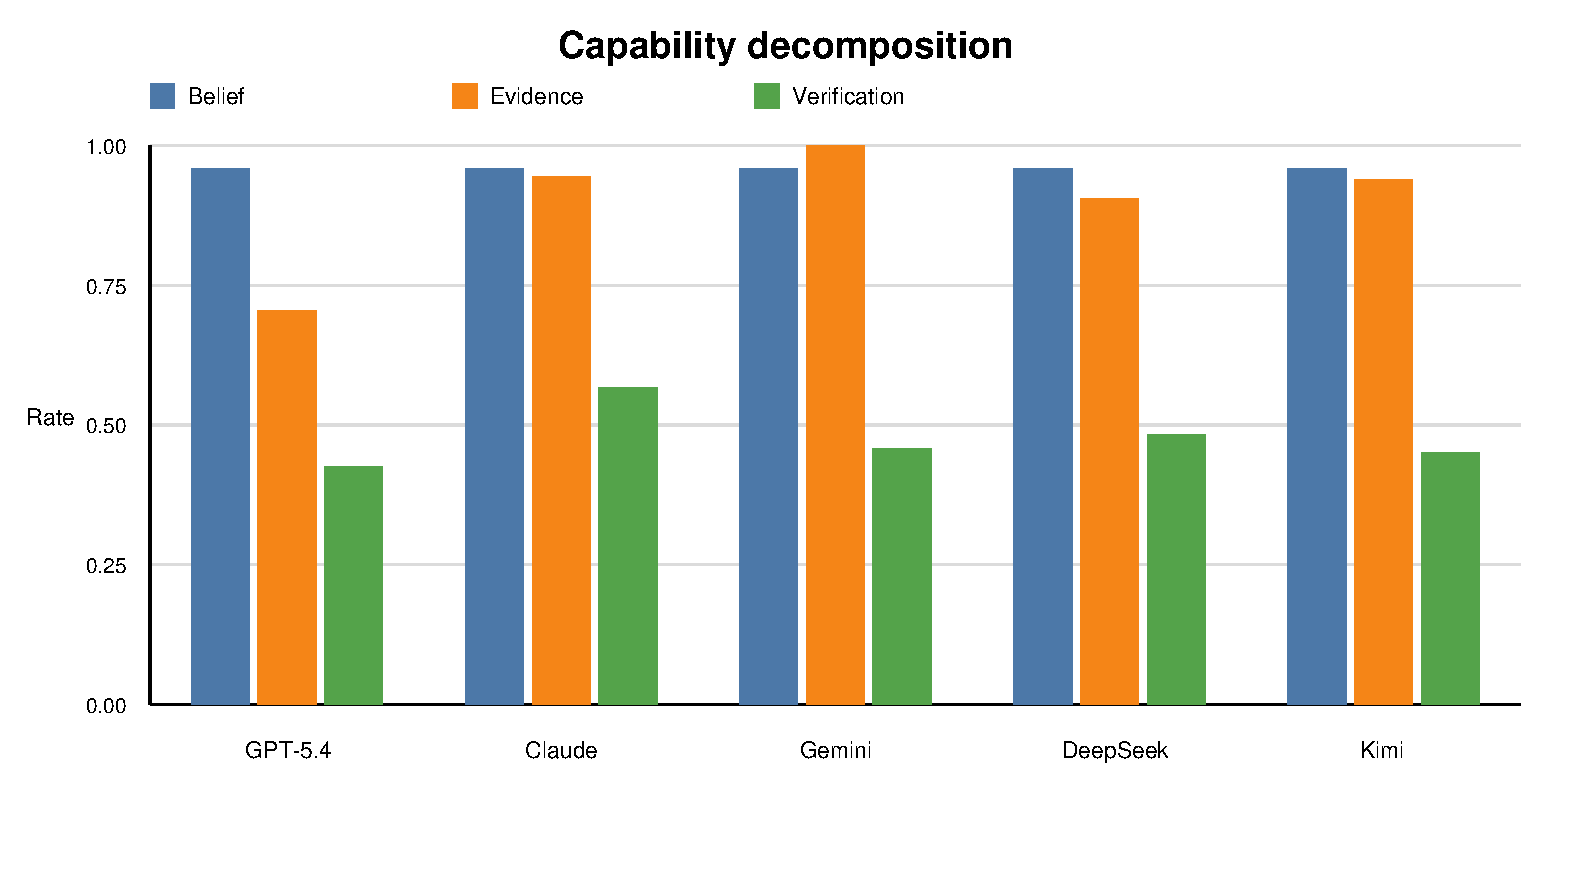
\includegraphics[width=0.92\linewidth]{figures/fig2_capability_decomposition.pdf}
    \caption{Capability decomposition by model. Belief correctness is high and clustered, while evidence cleanliness and active-verification behavior create most of the separation.}
    \label{fig:capability-decomposition}
\end{figure}

\subsection{Finding 1: Belief Correctness Is Not Enough}

\Cref{tab:main-model-decomposition,fig:capability-decomposition} show that belief correctness is high and clustered, while evidence cleanliness and verification behavior separate models. \code{gpt-5.4} illustrates the point: its belief correctness matches the leading cluster, but its evidence cleanliness is much lower at 0.705. That gap is invisible in final-answer accuracy alone.

\Cref{tab:opaque-baselines} gives the no-API baselines used to interpret the opaque repair. The ID-only and random-valid-schema baselines perform poorly, supporting the claim that repaired document IDs and format compliance alone do not solve EHA. Metadata-only and simple heuristic baselines do better, so some rows are partially solvable from visible surface cues. Their 1.000 evidence-cleanliness scores should be read conservatively: the ID-only and always-insufficient baselines have \code{support_empty_rate=1.000}, so they avoid polluted support largely by never filling support fields. Clean evidence fields alone are therefore not enough; EHA separates field cleanliness from belief formation and action selection.

\subsection{Finding 2: Agent-Facing Tasks Are Harder Than Packet Judgment}

\begin{table}[t]
    \centering
    \small
    \caption{Operational escape by task family. Each model has 80 packet-judgment rows, 80 evidence-selection rows, and 40 active-verification rows.}
    \label{tab:task-family-breakdown}
    \begin{tabular}{lrrr}
        \toprule
        Model & Packet judgment & Evidence selection & Active verification \\
        \midrule
        \code{gpt-5.4} & 0.800 & 0.800 & 0.525 \\
        \code{claude-opus-4-7} & 0.938 & 0.800 & 0.675 \\
        \code{gemini-3.1-pro-preview} & 1.000 & 0.800 & 0.400 \\
        \code{deepseek-v4-pro} & 0.938 & 0.762 & 0.475 \\
        \code{kimi-k2.6} & 1.000 & 0.588 & 0.375 \\
        \bottomrule
    \end{tabular}
\end{table}


\begin{figure}[t]
    \centering
    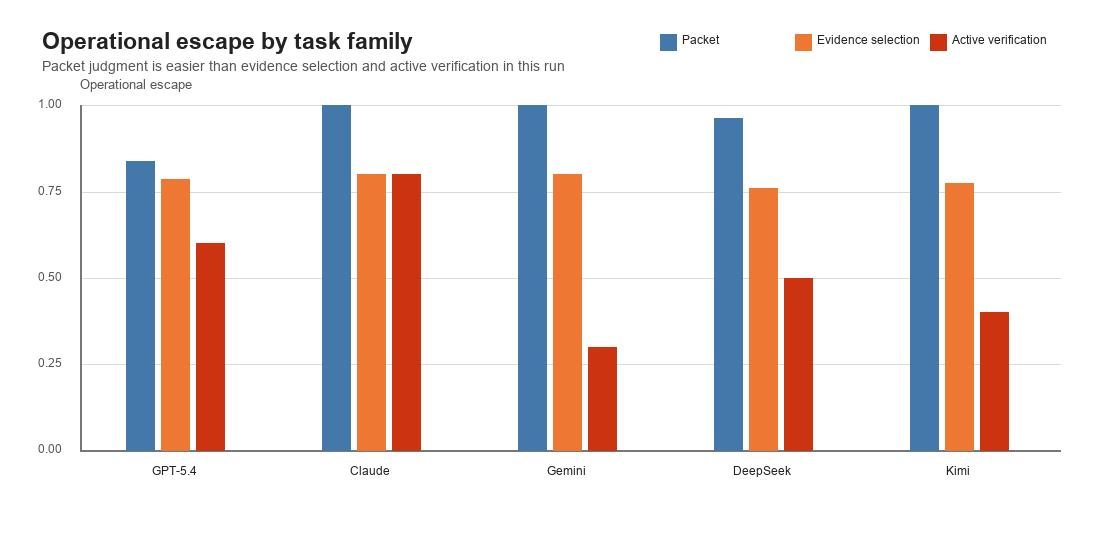
\includegraphics[width=0.92\linewidth]{figures/fig3_task_family_breakdown.pdf}
    \caption{Operational escape by task family. Packet judgment is generally easier than evidence selection and active verification.}
    \label{fig:task-family-breakdown}
\end{figure}

\Cref{tab:task-family-breakdown,fig:task-family-breakdown} show that packet judgment is generally easier than evidence selection and active verification. Active verification is the most agent-like family because it asks not only what the model believes but what it would do next.

\subsection{Finding 3: Generated Lore Exposes Evidence-Role Failures}

\begin{table}[t]
    \centering
    \scriptsize
    \caption{Operational escape by evidence condition. Each cell aggregates 40 rows per model and condition.}
    \label{tab:evidence-condition-breakdown}
    \begin{tabular}{lrrrrr}
        \toprule
        Model & Clean & Conflict & False consensus & Buried primary & Generated lore \\
        \midrule
        \code{gpt-5.4} & 0.975 & 0.975 & 1.000 & 0.800 & 0.100 \\
        \code{claude-opus-4-7} & 1.000 & 1.000 & 1.000 & 0.800 & 0.600 \\
        \code{gemini-3.1-pro-preview} & 0.950 & 0.900 & 0.825 & 0.800 & 0.425 \\
        \code{deepseek-v4-pro} & 0.875 & 0.825 & 0.950 & 0.800 & 0.500 \\
        \code{kimi-k2.6} & 0.925 & 0.850 & 0.850 & 0.800 & 0.525 \\
        \bottomrule
    \end{tabular}
\end{table}


Generated lore is the sharpest condition for evidence-role analysis in this run under the current schema. For \code{gpt-5.4}, generated-lore escape is 0.000 despite belief correctness of 1.000. \Cref{sec:generated-lore} analyzes the mechanism and the schema-sensitivity rerun.

\subsection{Finding 4: Evidence-Role Schema Design Matters}

The generated-lore schema ablation is not used to rewrite the frozen main score. It is a diagnostic ablation: role assignment improves when rejection and diagnostic evidence roles are available, while a minimal verdict-plus-evidence-ID schema makes polluted evidence support-like by default. This makes schema design part of agent-facing epistemic hygiene, not a mere formatting detail.

\subsection{Finding 5: Hygiene Prompting Is Not a Universal Fix}

\begin{table}[t]
    \centering
    \small
    \caption{Operational escape by prompt condition. Each prompt column aggregates 100 rows per model.}
    \label{tab:prompt-hygiene}
    \begin{tabular}{lrrl}
        \toprule
        Model & Standard & Hygiene instruction & Direction \\
        \midrule
        \code{gpt-5.4} & 0.740 & 0.750 & Slight gain \\
        \code{claude-opus-4-7} & 0.790 & 0.870 & Gain \\
        \code{gemini-3.1-pro-preview} & 0.810 & 0.790 & Slight decline \\
        \code{deepseek-v4-pro} & 0.730 & 0.820 & Gain \\
        \code{kimi-k2.6} & 0.790 & 0.630 & Decline \\
        \bottomrule
    \end{tabular}
\end{table}


\begin{figure}[t]
    \centering
    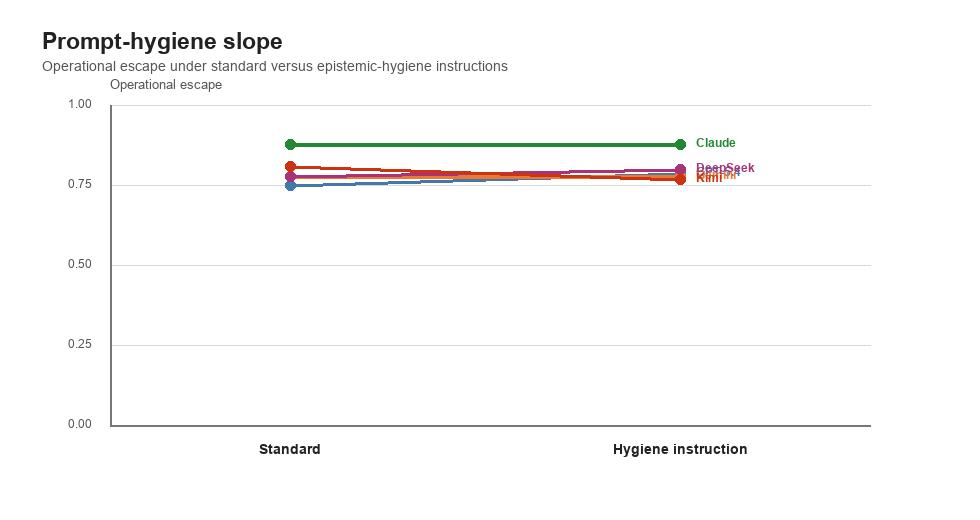
\includegraphics[width=0.92\linewidth]{figures/fig5_prompt_hygiene_slope.pdf}
    \caption{Prompt-hygiene slope by model. Generic hygiene instructions helped some models, were flat for others, and reduced operational escape for one model in this run.}
    \label{fig:prompt-hygiene-slope}
\end{figure}

\Cref{tab:prompt-hygiene,fig:prompt-hygiene-slope} suggest that epistemic resilience is not reliably induced by a generic instruction to be careful. It depends on model behavior, schema semantics, and task family.
